\documentclass[article]{beamer}
\beamertemplatenavigationsymbolsempty

\usepackage{tikz}

\begin{document}

\begin{frame}{Desired behavior}

\begin{itemize}[<+->]

\item Handout mode collapses these pauses into one slide
\item I expect this behavior and want it here
\item But I do not want it on the next frame
\item Imagine the following tikzpicture is very complicated
\item I want to make small changes, shown as separate slides
\item I want these to remain as separate slides in handout mode
\item How to accomplish this? Thanks!

\end{itemize}
\end{frame}

\begin{frame}{Desired behavior in handout mode}

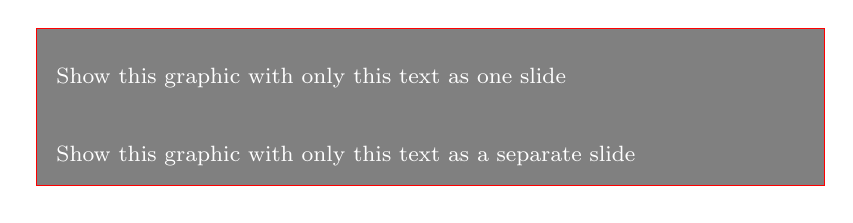
\begin{tikzpicture}

\draw[draw=red,fill=gray] (0,0) rectangle (10,2);

\onslide<1>{
  \node[label={[font=\footnotesize,text=white]45:{Show this graphic with only this text as one slide}}] at (0,1) {};
}

\onslide<2>{
  \node[label={[font=\footnotesize,text=white]45:{Show this graphic with only this text as a \alert{separate} slide}}] at (0,0) {};
}

\end{tikzpicture}
\end{frame}

\end{document}
